Using the \intlumiSevenTeV\ and \intlumiEightTeV\ of data collected by the CMS detector 
in 2011 and 2012 at 7 and 8~\TeV\ center of mass energy, respectively, we have performed 
a search for the standard model Higgs boson in the range \mHi=110 - 600~\GeV\ 
and a study on its spin-parity nature at \mHi=125~\GeV\ 
in the full leptonic final states of $W^+W^-$ decay mode. 
The analysis is performed in the 4 categories divided by the lepton flavor and the 
number of jets because the composition of background is different
in the different categories. 

There are two neutrinos in the final state, so \mHi\ is not be able to be reconstructed, 
thus not measured. We measure an overall excess on top of backgrounds, 
therefore an accurate and precise 
estimation of backgrounds is the key in this analysis. For the reliable estimation 
of the major backgrounds, we apply date-driven methods to all major backgrounds. 
%
A new analysis method which uses the 2-dimensional templates of \mT\ and \mll\ has been developed,
and enhanced the search sensitivity of \mHi=125~\GeV\ SM Higgs boson by 25~\%. 
The new method is used only in the \DF\ category because of the poor modeling of \dyll\
template in the \SF\ category. The cut-based method is used in the \SF\ category.
%
The new analysis uses templates constructed using simulation, and we 
validate the fit model of the major backgrounds using dedicated control 
regions in data. 

The expected exclusion limit of the SM Higgs at $\CLs=95~\%$ is $115-575~\GeV$, 
and we observe an excess in the low \mHi\ region giving the observed exclusion 
limit $128-600~\GeV$. 
The excess of the data is quantified in terms of imcompatibility of the 
\textit{background-only} hypothesis. The expected signifance at \mHi=125~\GeV\ 
is 5.2$\sigma$, and we observe $4.0\sigma$.
The production rate is measured in the unit of expected $\sigma \times BR$ in SM, 
and the measured rate is $0.76 \pm 0.13(stat.) \pm 0.16(syst.)$.  

The spin-parity nature of the new boson has been tested by performing hypothesis 
tests using a graviton-like spin-2 and a psedu-scalar spin-0 models. The data 
favors SM Higgs to the spin-2 and spin-0 models by \CLs=0.2-16.3~\% and 34.7 \%, 
respectively.
\\

The result of this analysis was used for the historic discovery of the new boson 
and understanding of its spin-parity nature. In the July 2012, the CMS and 
the ATLAS collaborations announced the discovery of a new boson~\cite{Chatrchyan:2012ufa,Aad:2012tfa}
around \mHi=125~\GeV, which led to the Nobel Prize in Physics in 2013. 
\begin{figure}[htp] 
\centering 
\begin{tabular}{c} 
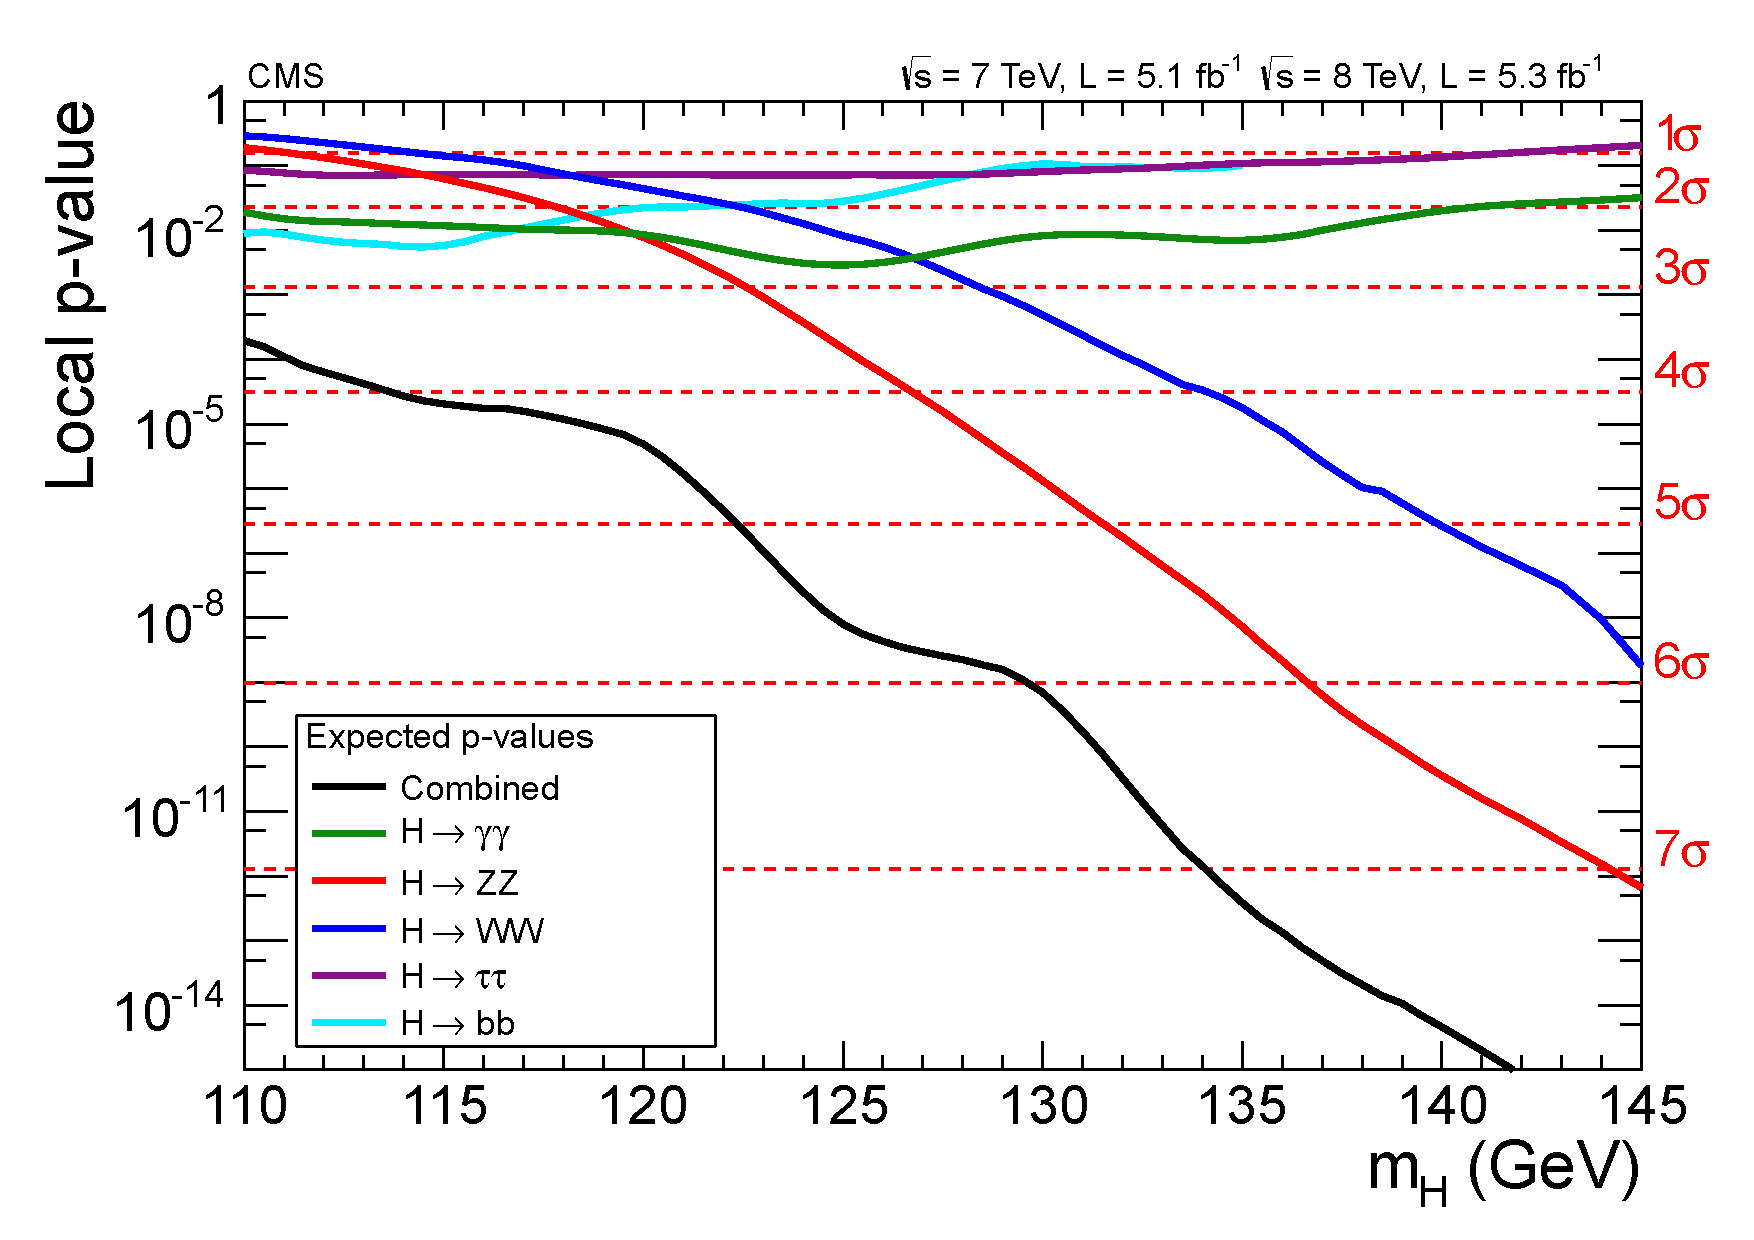
\includegraphics[width=0.45\textwidth]{figures/fig1.pdf} 
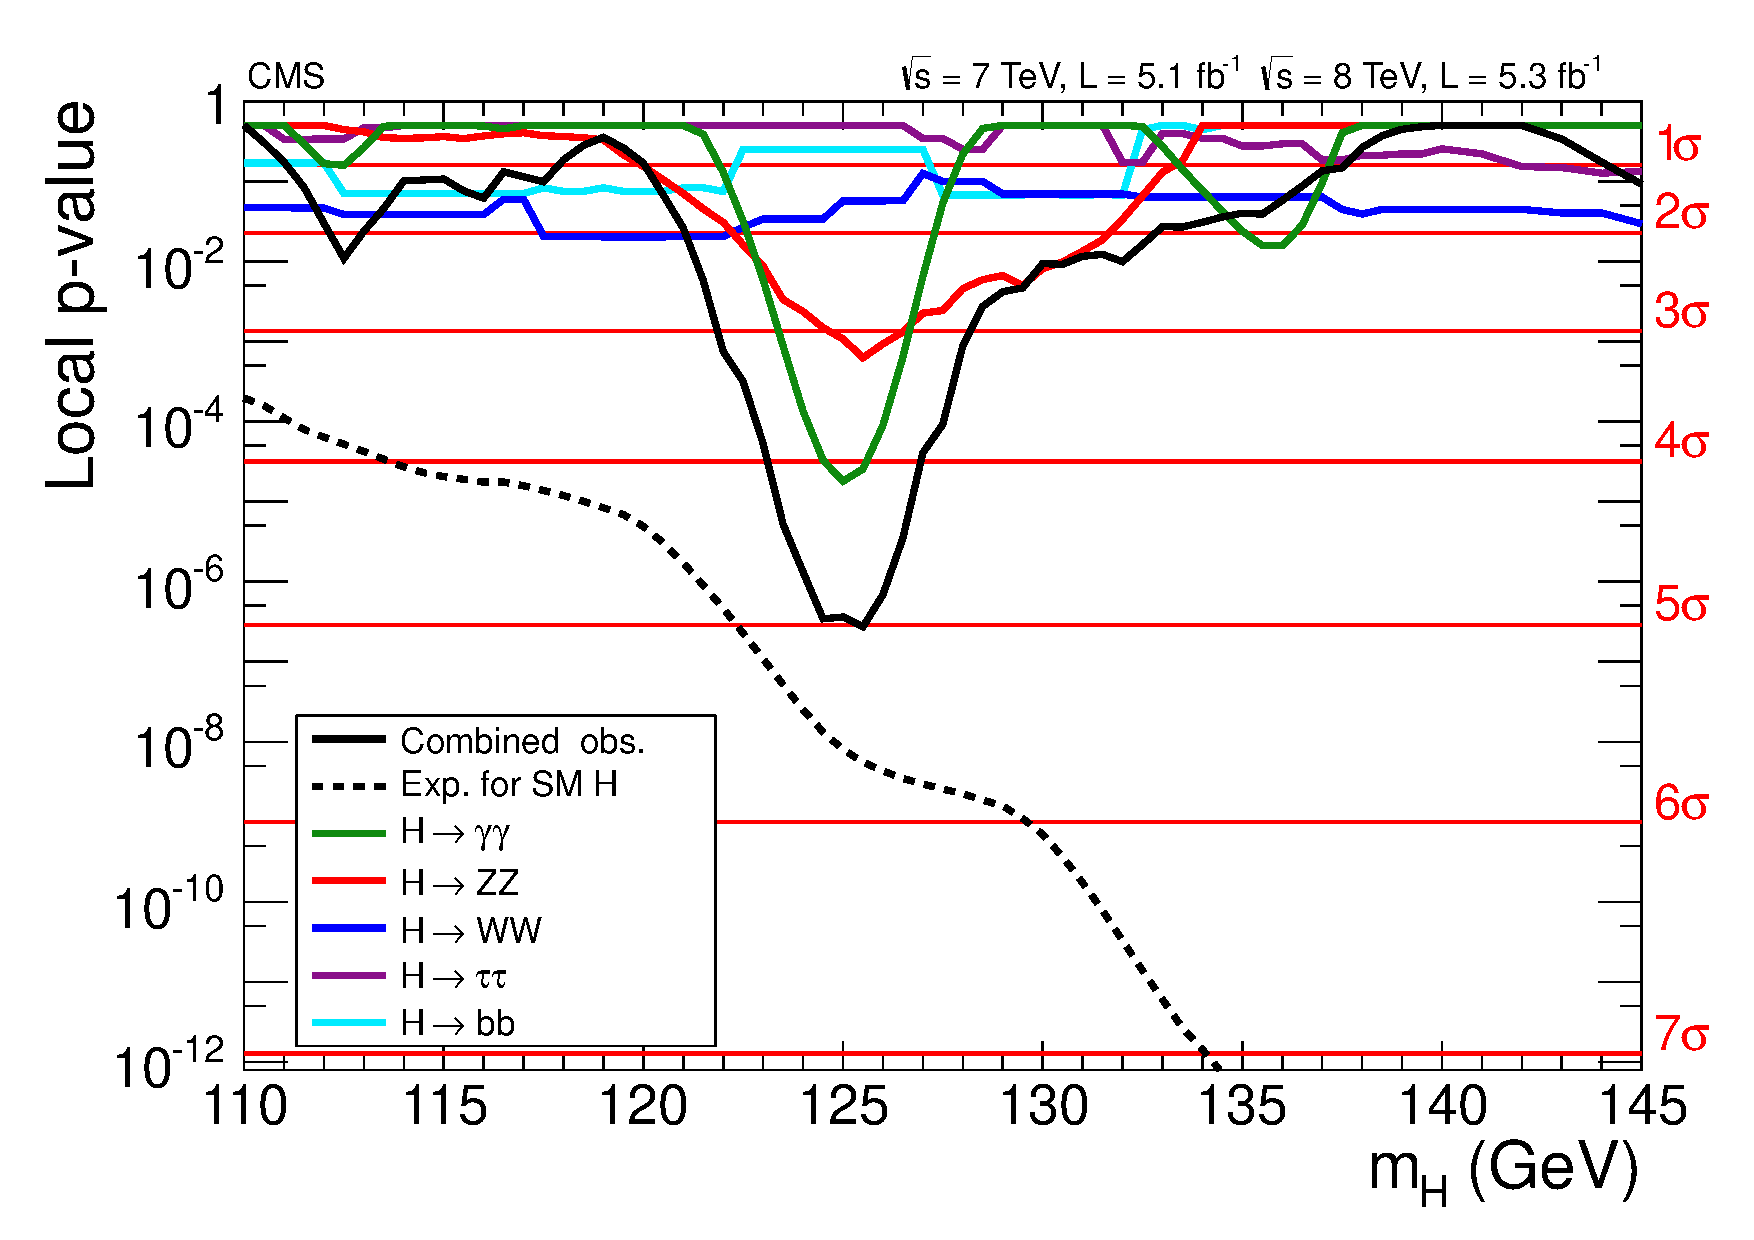
\includegraphics[width=0.45\textwidth]{figures/fig15.pdf} 
\end{tabular} 
\caption{Expected(left) and observed(right) significance using data collected by July 2012.} 
\label{fig:ichep2012} 
\end{figure} 
Figure~\ref{fig:ichep2012} shows the expected and observed significance from 
the all data available in July 2012. The \hww\ mode has a good sensitivity 
in the higher mass region, but at the mass point where the new boson was 
discovered, the excess is about $2\sigma$. This analysis was used to 
exclude large range of high mass region, and narrowed down the search window
to the low \mHi\ region. 

Using the full data collected in 2011 and 2012, the signal strength 
was measured combining all channels~\cite{CMS-PAS-HIG-13-005}. 
\begin{figure}[htp] \centering 
\begin{tabular}{c} 
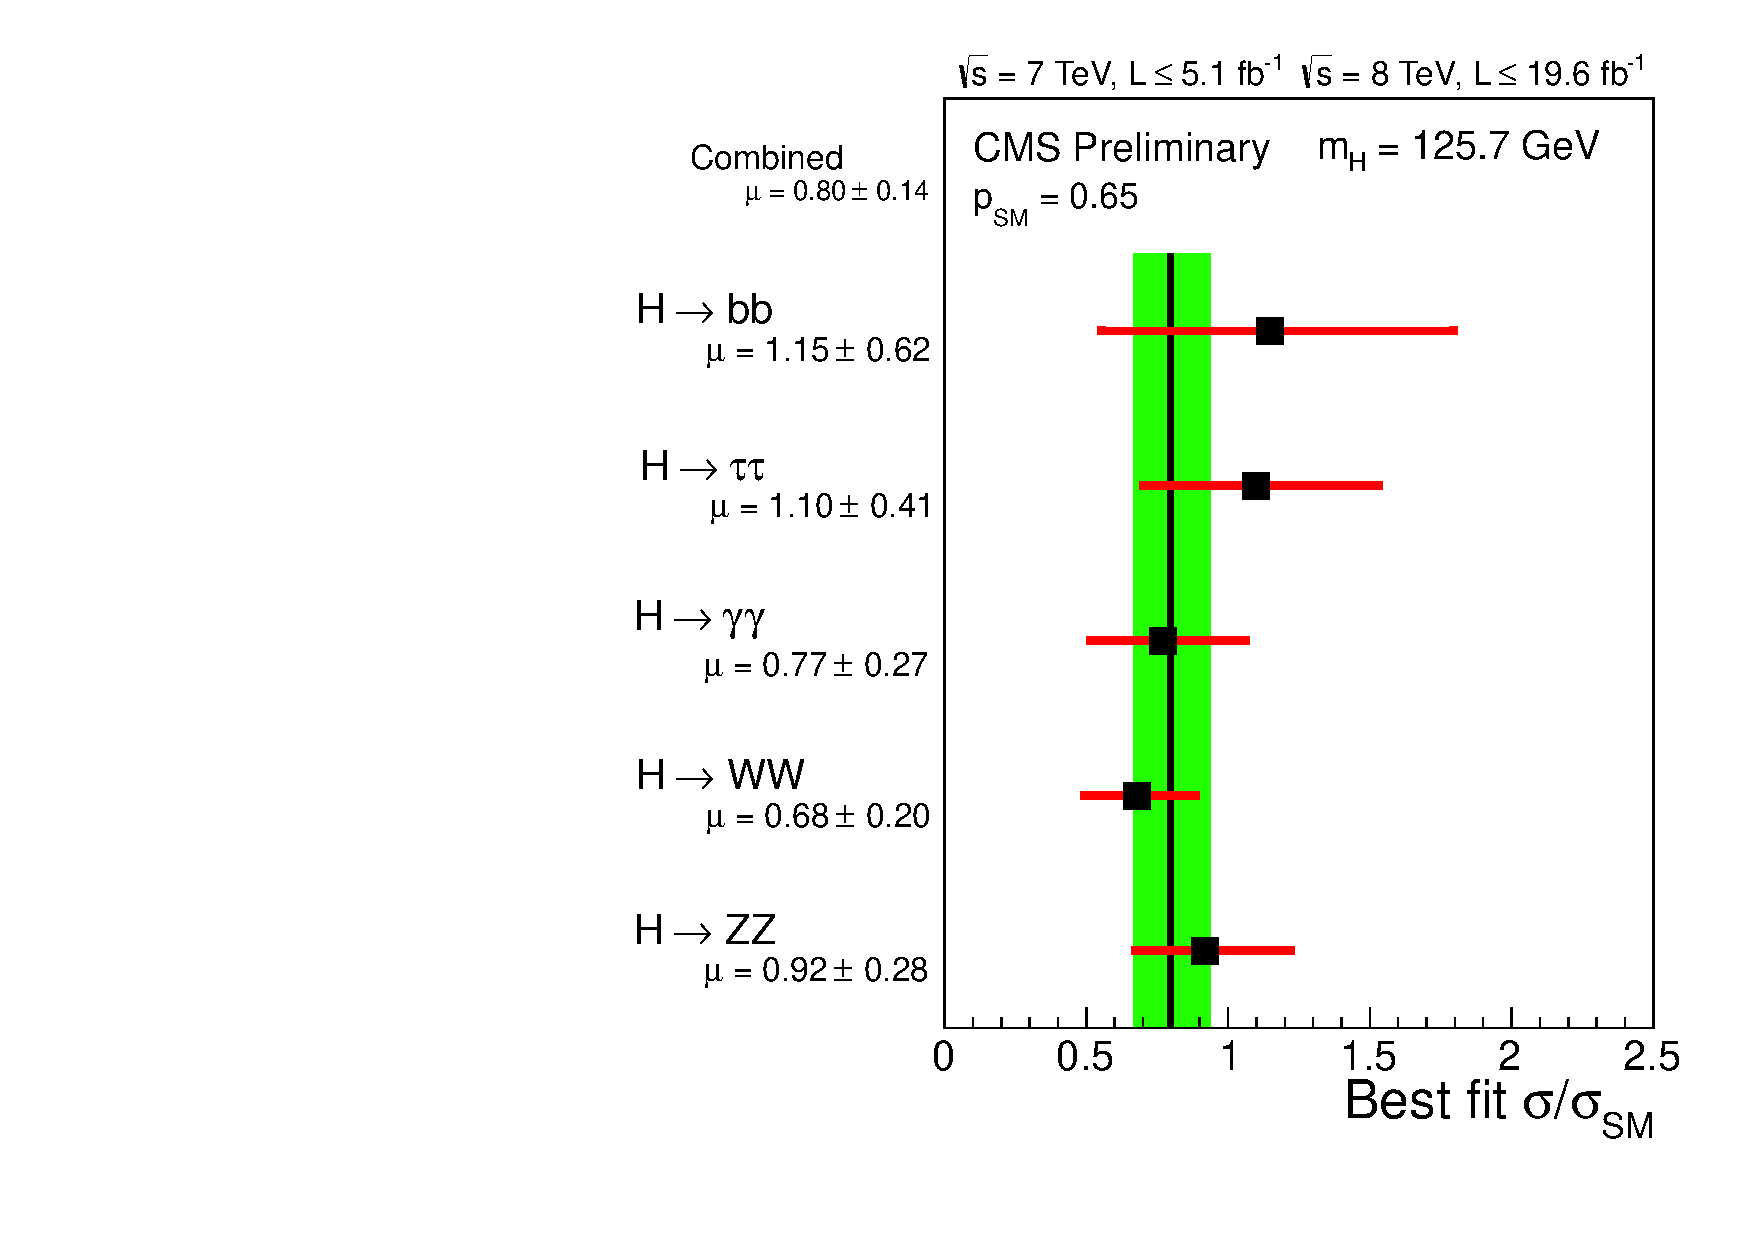
\includegraphics[width=0.8\textwidth]{figures/sqr_mlz_ccc_mH125_7_decay.pdf} 
\end{tabular} 
\caption{Signal strength measured by the five most sensitive channels. 
The black line and the green bands shows the combined measurement, 
$\mu = 0.80 \pm 0.14$.} 
\label{fig:mucomb} 
\end{figure} 
Figure~\ref{fig:mucomb} shows the signal strength measured at \mHi=125.7~\GeV\
by the five most sensitive channels. The \hww\ channel measures the signal strength
at the best precision. 

The spin-parity study on the spin-2 model was combined with the \hzz\ channel.  
\begin{figure}[htp] \centering 
\begin{tabular}{c} 
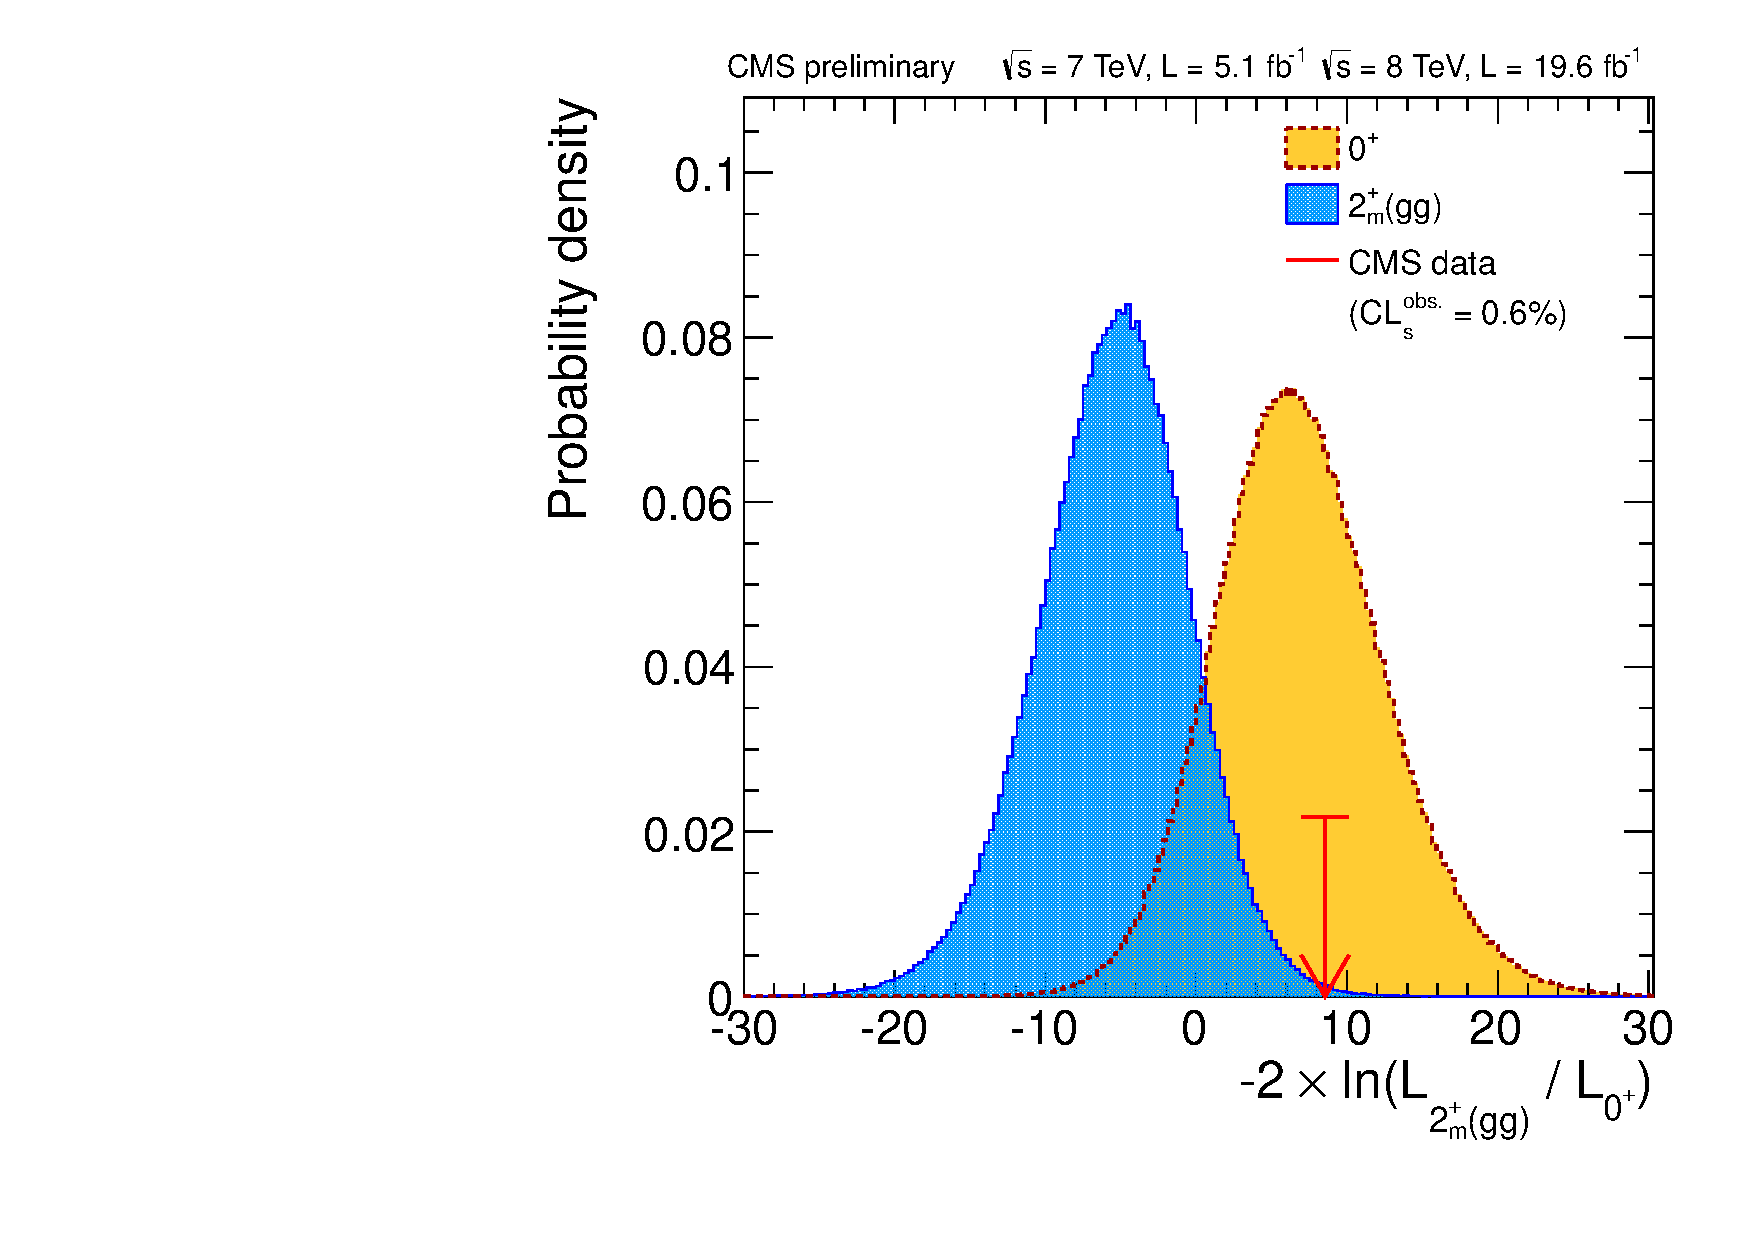
\includegraphics[width=0.8\textwidth]{figures/hvv_a-posteriori_qvals_root_2pmgg.pdf} 
\end{tabular} 
\caption{Distribution of $q_{2_{min}^+}$ assuming $0^+$ and $2_{min}^+$ models.  
Blue is the expected distribution assuming $2_{min}^+$, 
and orange is the expected distribution assuming $0^+$ hypothesis.
The plot shows the result using the best-fit value of the signal strength.}  
\label{fig:spincomb} 
\end{figure} 
Figure~\ref{fig:spincomb} shows the $q_{2_{min}^+}$ distrbutions in case the spin-2 resonance 
is produced via gluon-gluon interaction. The combined result shows that the 
expected and the observed exclusion of the spin-2 model are \CLs=1.2~\% and 0.6~\%, 
respectively. 
\\ 

In conclusion, the Higgs boson, the last piece of the standard model, 
was discovered in July 2012, and \hww\ channel made a significant contribution 
to the discovery by excluding the SM Higgs hypothesis in the high \mHi\ region. 
The measured production rate and the test on the spin-parity shows 
that the new boson is compatible with the SM Higgs boson at \mHi=125~\GeV.  
